\chapter{BSW Modules Configuration Hints}
\label{chap:bswconfig}

This chapter provides a guideline about the expected configuration of some of the BSW Modules interacting with SSFM.

\section{BswM configuration}
N/A
\section{Com Configuration}
The integrator will need to Configure the "ComNotification" to the one of the RTE and "ComTimeoutNotification" to the specific one Sum\_Ssfm\_COMCbkTOut\_<SerialData> for the relevant Rx messages in Com. See example below (the notification functions can have any relevant name):

\begin{figure}[H]
	\centering
	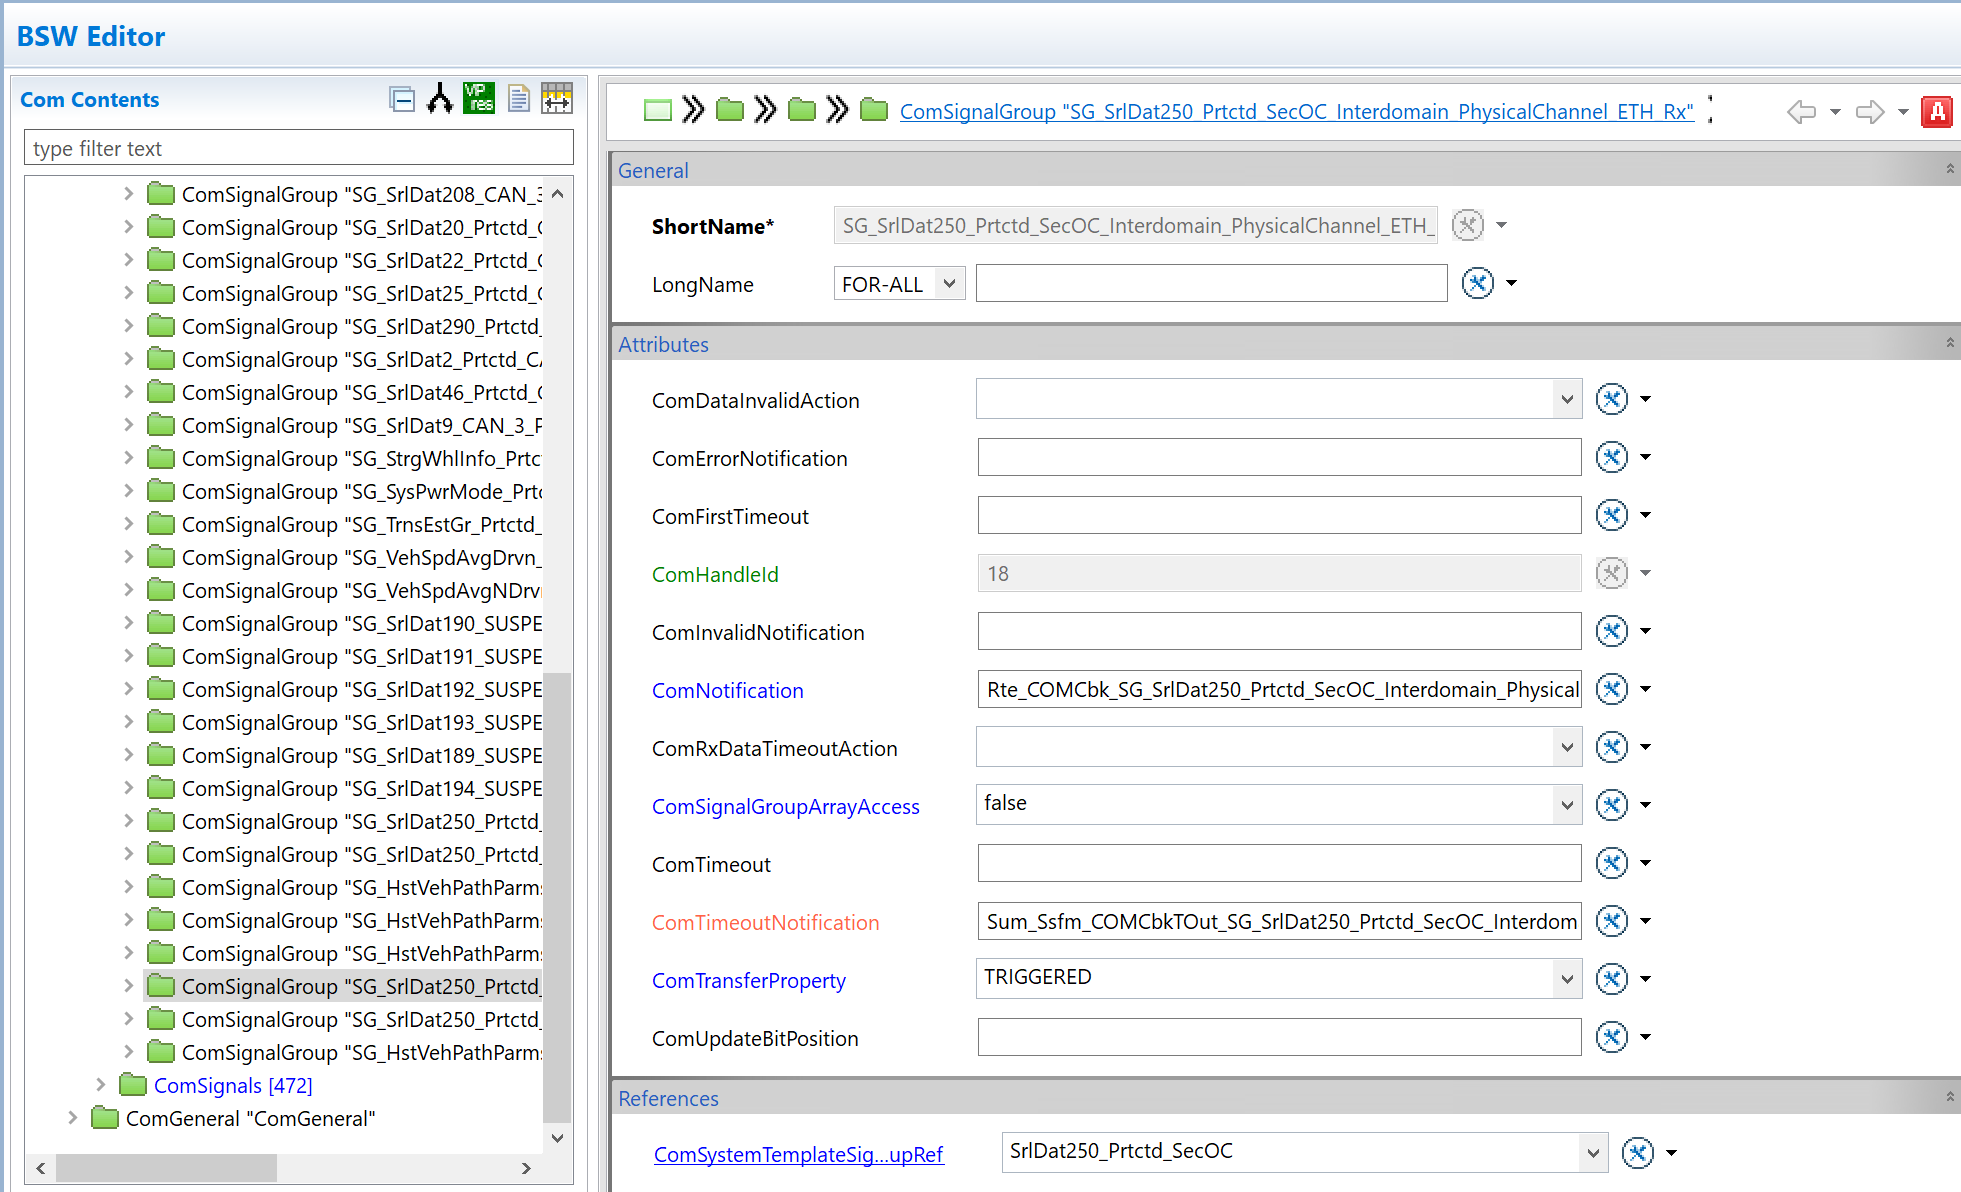
\includegraphics[scale=0.35]{images/comConfig.png}
\end{figure}

\section{Dem Configuration}
\label{sec:DemConf}
The integrator should configure the DemEventParameter properly for the U19A3 57 failure aggregation.
The name of the DemEventParameter should follow the following pattern: \code{DTC_#FTB#_Event}.
For instance for DTC U19A3 57 the DemEventParameter name should be configured as: \\\code{DTC_U19A3_57_Event}
\begin{figure}[H]
	\centering
	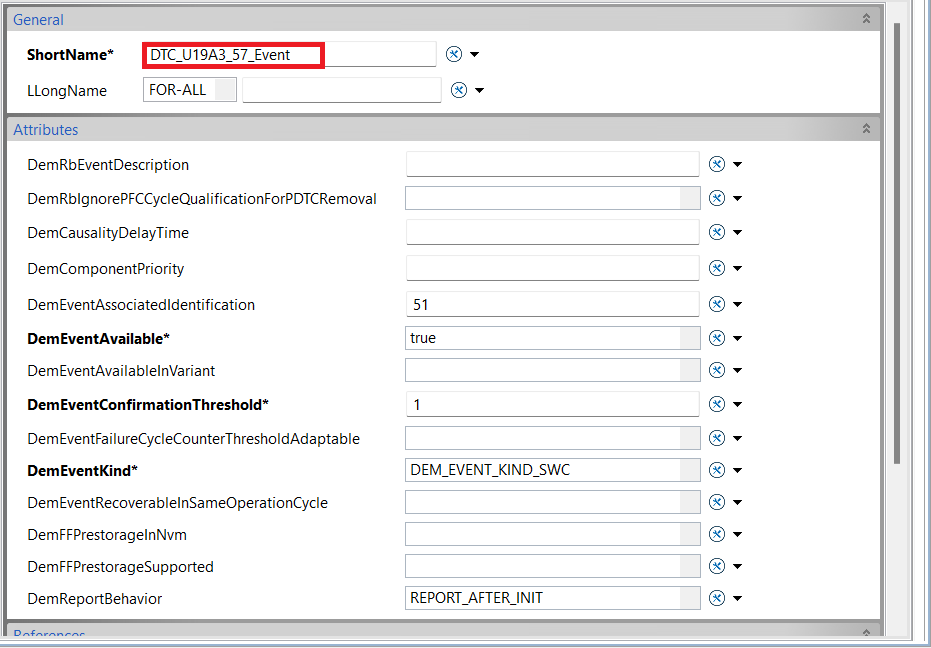
\includegraphics[scale=0.35]{images/DTC_U19A3_57.png}
\end{figure}

The integrator should configure the DemEventParameter properly for the U19A3 92 failure handler.
The name of the DemEventParameter should be the following: \code{DTC_U19A3_92_Event}
\begin{figure}[H]
	\centering
	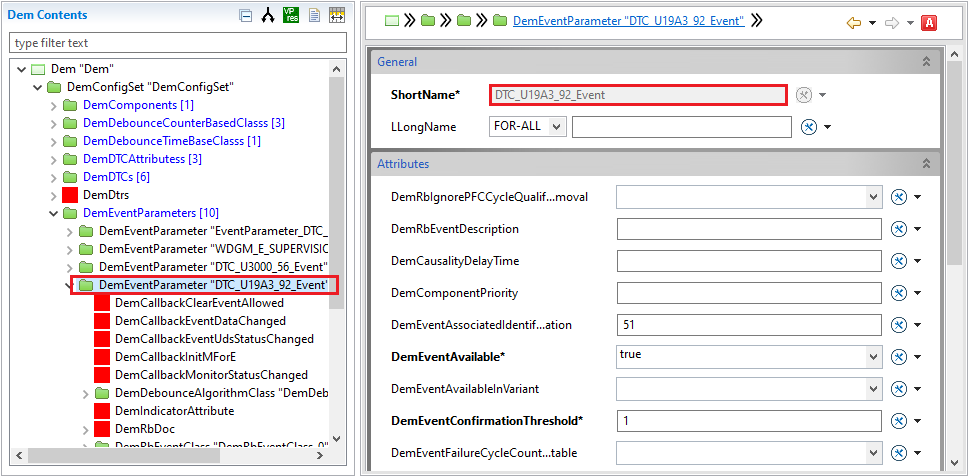
\includegraphics[scale=0.35]{images/DTC_U19A3_92_dem_configuration.png}
\end{figure}

\section{Dcm Configuration}
\label{sec:DcmConf}
The integrator should configure the "DcmDsdServiceRequestSupplierNotification" to define the name of the R-Port through which the DCM accesses the interface ServiceRequestNotification for the Service 0x14 Handler.

\begin{figure}[H]
	\centering
	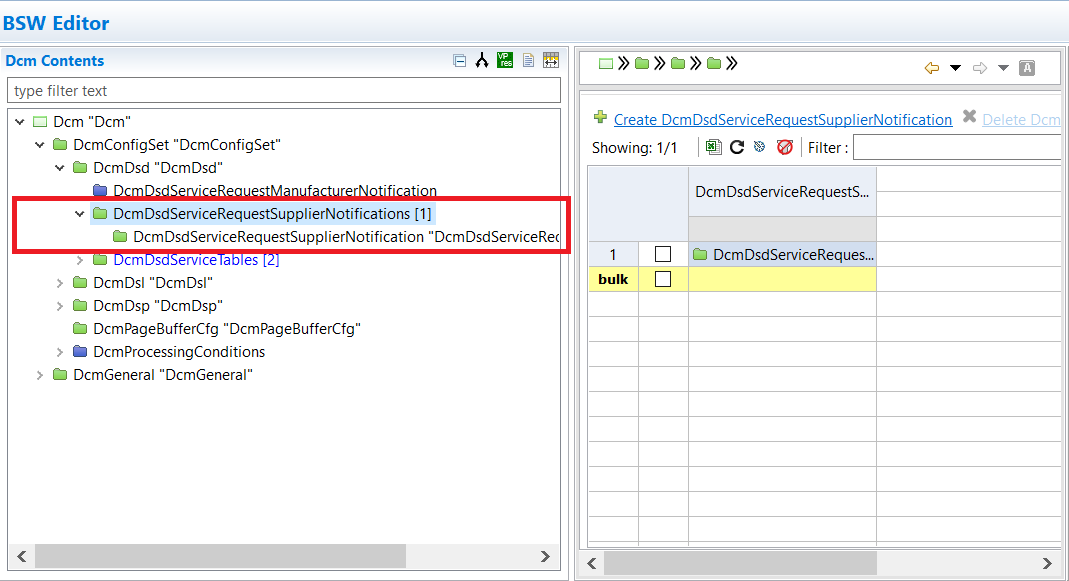
\includegraphics[scale=0.35]{images/DcmConfiguration.png}
\end{figure}

\section{NvM Configuration}
\label{sec:NvMConf}

The integrator can use the static file Sum\_Ssfm\_ServiceNeeds.arxml together with the BSW ConfGen to automatically generate the NvM blocks and Per Instance Memory ram instances needed by the SSFM.
If a block is not needed, ex. DID F094 since SOH is not integrated, then the integrator can safely remove the relatives Service Need, AR Typed Per Instance Memory and Implementation Data Type in the mentioned file. 